% RIPE-Select (ORB/BRISK) — CVPR 2025 author kit (cvpr.sty v3.1), camera-ready layout with page numbers.
% Build: pdflatex --include-directory=texmf main ; bibtex main ; pdflatex x2   (texmf/ holds vendored packages)
\documentclass[10pt,twocolumn,letterpaper]{article}
\usepackage[pagenumbers]{cvpr}

\usepackage{microtype}
\usepackage{multirow}
\usepackage{tikz}
\usetikzlibrary{arrows.meta,positioning,fit,backgrounds,calc}
\usepackage[detect-weight=true,detect-family=true,mode=text,separate-uncertainty=true,
            table-align-uncertainty=true]{siunitx}

\definecolor{cvprblue}{rgb}{0.21,0.49,0.74}
\usepackage[pagebackref,breaklinks,colorlinks,allcolors=cvprblue]{hyperref}
\usepackage[capitalize,nameinlink]{cleveref}

% ---- palette (same hex values as proj/scripts/paper_figures.py)
\definecolor{ours}{HTML}{6F4E9C}
\definecolor{vanilla}{HTML}{3A6FB0}
\definecolor{grid}{HTML}{2E9E77}
\definecolor{baseline}{HTML}{5E5E5E}
\definecolor{good}{HTML}{1FA35B}
\definecolor{bad}{HTML}{E05A1B}

% ---- macros
\newcommand{\ours}{\textup{\textsc{Ripe-Select}}\xspace}
\newcommand{\B}[1]{\bfseries #1}
\newcommand{\U}[1]{\underline{#1}}
\newcommand{\q}[1]{\noindent\textbf{#1}\hspace{0.4em}}
\newcommand{\finding}[1]{\par\smallskip\noindent\colorbox{ours!8}{\parbox{\dimexpr\linewidth-2\fboxsep}{\small
  \textcolor{ours}{\textbf{Finding.}} #1}}\par\smallskip}
\newcounter{algo}
\makeatletter\newcommand{\tabinput}[1]{\@@input #1 }\makeatother
\crefname{algo}{Algorithm}{Algorithms}
\graphicspath{{figures/}}

\def\paperID{*****}
\def\confName{CVPR}
\def\confYear{2025}

\title{Which Keypoints Should ORB Keep?\\
Learning Classical Keypoint Selection from Image-Pair Labels}

\author{Anonymous submission}

\begin{document}

% ============================================================================ teaser
\twocolumn[{%
\renewcommand\twocolumn[1][]{#1}%
\maketitle
\vspace{-1.6em}
\begin{center}
  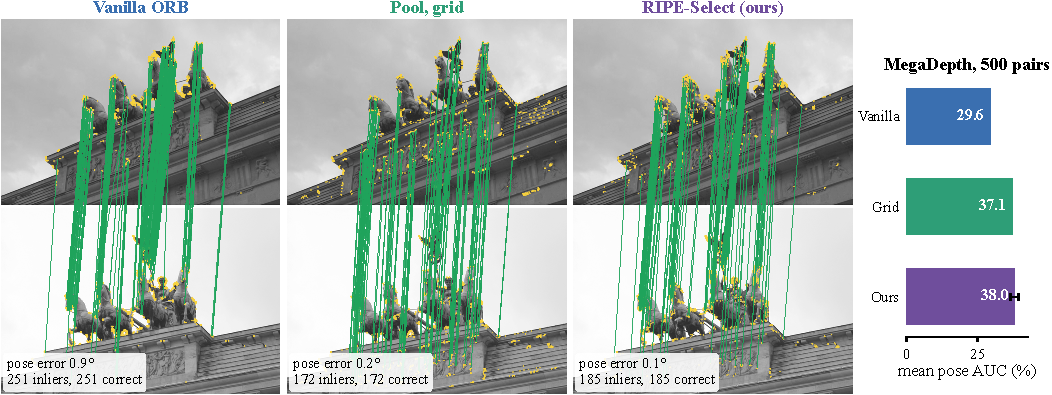
\includegraphics[width=\textwidth]{teaser.pdf}
  \captionof{figure}{\textbf{Same detector, same descriptor, same budget---different keypoints.} ORB on a
  MegaDepth pair, keeping $K{=}2048$ keypoints (yellow) with OpenCV's response ranking, a spatial grid, or our
  learned policy. Lines are a random subset of 70 RANSAC inliers, \textcolor{good}{green} if geometrically correct
  and \textcolor{bad}{orange} otherwise. The pair is not hand-picked: its gain is the closest to the mean gain over
  all 500 test pairs. Right: mean pose AUC over the benchmark (\ours: five seeds).}
  \label{fig:teaser}
\end{center}
\vspace{0.6em}
}]

% ============================================================================ abstract
\begin{abstract}
Since their introduction, classical detectors such as ORB and BRISK have decided which keypoints to keep the same way:
the $K$ with the highest corner response. We show that this choice is worth learning. Response barely predicts
which keypoints will match, and a small policy trained only with RIPE's image-pair reward---a kept keypoint
scores when its match survives RANSAC on a same-scene pair and is penalised on a different-scene pair---picks
much better ones. \ours leaves the detector, the binary descriptor, the matcher and RANSAC untouched; it only
re-ranks the detector's own candidates. Trained on two scenes on a laptop CPU, it raises MegaDepth-1500 pose
AUC from 29.6 to \textbf{38.0} for ORB (+8.5, AUC@5$^\circ$ \textbf{+31\,\%} relative) and from 41.5 to
\textbf{46.0} for BRISK. Every one of five training seeds
improves significantly, and ORB with learned selection overtakes a learned binary feature reported in the
literature. Analysing the policy, we find that it swaps two-thirds of the kept keypoints, ignores the detector
response, and gains pose accuracy not by finding more correct matches but by spreading them over the image---a
lesson it learns from a per-keypoint reward without ever seeing image coordinates.
\end{abstract}

% ============================================================================ intro
\section{Introduction}
\label{sec:intro}

Learned local features~\cite{detone2018superpoint,tyszkiewicz2020disk,zhao2023aliked,kunzel2025ripe} have
advanced image matching rapidly, yet classical features remain what a large share of deployed systems run.
ORB~\cite{rublee2011orb} is the front end of ORB-SLAM~\cite{murartal2015orbslam}; binary features are the
default wherever compute, memory, power or licensing are tight, and even recent ``fast'' learned
features~\cite{potje2024xfeat,kanakis2023zippypoint} are benchmarked against them. All of these pipelines share
one step that has not changed since they were proposed: detect many candidates, then keep the $K$ with the
highest detector response.

\q{Response is the wrong criterion.} Response measures local contrast, not \emph{matchability}. On MegaDepth,
response separates candidates that end in a correct match from those that do not with a ROC-AUC of only
0.56--0.60, the correct-match rate barely falls from the strongest to the weakest response quartile, and a
top-$K$ cut by response throws away more than half of the correct matches present among the candidates
(\cref{fig:matchability}). Which $K$ keypoints to keep is therefore an open, cheap and so far unexploited lever.

\q{Learning the choice without labels.} RIPE~\cite{kunzel2025ripe} trains a keypoint detector by reinforcement
learning from nothing more than whether two images show the same scene. A classical detector has no heatmap to
sample from, so we learn a \emph{selection policy} over its candidates instead (\cref{fig:method}). A small MLP
scores every candidate from local cues and its descriptor; a budget-exact Bernoulli selection keeps exactly $K$ in
expectation; RANSAC on same-scene and different-scene pairs supplies the reward. Detector, descriptor, matcher
and robust estimator are unchanged, so \ours is a drop-in module.

\q{What we find.} Under a controlled protocol in which every method shares images, candidates, budget,
descriptor, matcher and RANSAC, learned selection improves ORB and BRISK at every pose threshold on
MegaDepth-1500 (\cref{fig:landscape}): +8.5 and +4.5 mean pose AUC, every seed significant. Opening the policy
up, we find that it replaces about two-thirds of the response-ranked keypoints and that its gain comes from
\emph{where} the matches land more than from \emph{how many} are correct: the policy discovers spatial spread
on its own, the property that the grid bucketing of ORB-SLAM imposes by hand.

\begin{figure}[t]
  \centering
  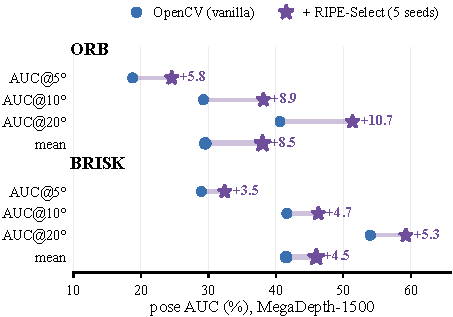
\includegraphics[width=\linewidth]{landscape.pdf}
  \caption{\textbf{Same detector, same descriptor, better keypoints.} Pose AUC on MegaDepth-1500 for OpenCV's
  response ranking and for \ours selection from the detector's own candidates (mean of five seeds); labels: gain
  in AUC points.}
  \label{fig:landscape}
\end{figure}

\q{Contributions.}
\begin{itemize}[nosep,leftmargin=*]
  \item \ours, a keypoint selection policy for classical detectors trained with RIPE's pair-label reward, with a
        budget-exact Bernoulli selection that removes RIPE's keypoint-count regulariser (\cref{sec:method}).
  \item A controlled evaluation with five seeds, paired tests and published reference numbers, showing
        +8.5 (ORB) and +4.5 (BRISK) pose AUC over OpenCV on MegaDepth-1500 (\cref{sec:results}).
  \item An analysis of what the policy learns---which cues it uses, which keypoints it swaps and why the swap
        helps---and how it compares with the spatial grid (\cref{sec:analysis}).
\end{itemize}

% ============================================================================ method figure
\begin{figure*}[t]
\centering
\begin{tikzpicture}[
    font=\footnotesize, >={Stealth[length=4pt]},
    thumb/.style={inner sep=0pt, draw=black!25, line width=0.4pt},
    thcap/.style={font=\scriptsize, align=center, text width=2.1cm},
    proc/.style={draw, rounded corners=2pt, align=center, minimum height=1.05cm, inner sep=3pt, line width=0.6pt},
    frozen/.style={proc, fill=black!5, draw=black!45},
    learned/.style={proc, fill=ours!12, draw=ours, line width=0.9pt},
    arr/.style={->, line width=0.7pt, black!70},
    node distance=0.5cm]
  % ---- row 1: inference path
  \node[thumb] (img) {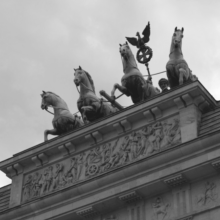
\includegraphics[width=1.55cm]{thumb_image.png}};
  \node[thcap, below=2pt of img] {image};
  \node[frozen, right=of img] (det) {OpenCV\\detector\\{\scriptsize lowered thr.}};
  \node[thumb, right=of det] (pool) {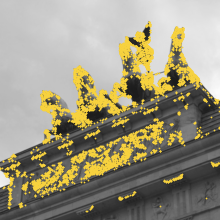
\includegraphics[width=1.55cm]{thumb_pool.png}};
  \node[thcap, below=2pt of pool] {candidate pool\\$4K$ + descriptors};
  \node[frozen, right=of pool] (cue) {20 cues + \\descriptor bits\\{\scriptsize no $(x,y)$}};
  \node[learned, right=of cue] (mlp) {MLP\\$s_i$};
  \node[learned, right=of mlp, text width=2.25cm] (sel)
        {keep $i$ w.p.\\$p_i=\sigma(s_i{+}b)$\\{\scriptsize $b$ s.t. $\sum_i p_i = K$}};
  \node[thumb, right=of sel] (kept) {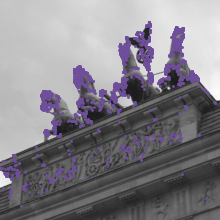
\includegraphics[width=1.55cm]{thumb_kept.png}};
  \node[thcap, below=2pt of kept] (keptcap) {$K$ kept\\(test: top-$K$ by $s_i$)};
  \foreach \a/\b in {img/det, det/pool, pool/cue, cue/mlp, mlp/sel, sel/kept} \draw[arr] (\a) -- (\b);
  % ---- row 2: training reward (matching block directly under the MLP)
  \node[proc, fill=white, draw=black!40, text width=2.3cm, font=\scriptsize] (match)
        at ($(mlp.south)+(0,-2.35)$) {MNN matching +\\F-RANSAC (1.5\,px)\\on kept keypoints};
  \node[thumb, right=0.6cm of match] (pos) {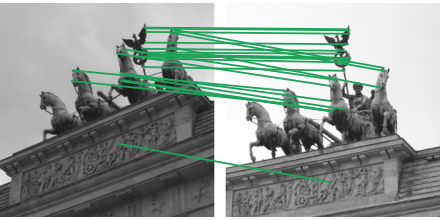
\includegraphics[width=2.1cm]{thumb_pos.png}};
  \node[thumb, right=1.1cm of pos] (neg) {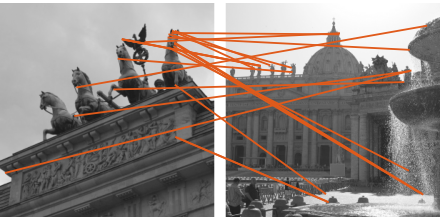
\includegraphics[width=2.1cm]{thumb_neg.png}};
  \node[font=\scriptsize, above=1pt of pos, align=center, text=good!70!black] (poslab)
        {same scene\\inlier $\Rightarrow r_i = +1$};
  \node[font=\scriptsize, above=1pt of neg, align=center, text=bad!80!black] (neglab)
        {other scene\\inlier $\Rightarrow r_i = -1$};
  \draw[arr] (keptcap.south) -- (keptcap.south |- neglab.north);
  \draw[arr] (pos.west) -- (match.east);
  \draw[arr, dashed, ours, line width=0.9pt] (match.north) -- (mlp.south)
        node[midway, right, font=\scriptsize, text=ours, align=left] {REINFORCE\\(\cref{eq:reinforce})};
  % ---- groups
  \begin{scope}[on background layer]
    \node[fit=(det)(cue)(pool), inner sep=5pt, rounded corners=4pt, fill=black!2, draw=black!20,
          label={[font=\scriptsize\itshape, black!55]above:frozen classical front end}] {};
    \node[fit=(mlp)(sel), inner sep=5pt, rounded corners=4pt, fill=ours!4, draw=ours!35,
          label={[font=\scriptsize\itshape, ours]above:learned (\ours)}] {};
    \node[fit=(match)(pos)(neg)(poslab)(neglab), inner sep=5pt, rounded corners=4pt, fill=black!2,
          draw=black!20, label={[font=\scriptsize\itshape, black!55]below:reward (training only)}] {};
  \end{scope}
\end{tikzpicture}
\caption{\textbf{\ours.} A classical detector run with lowered thresholds proposes a candidate pool; an MLP
scores every candidate from 20 local cues and its descriptor, without image coordinates. During training each
candidate is kept by a Bernoulli draw whose per-image bias $b$ fixes the expected count to the budget $K$; kept
keypoints are matched and earn $+1$ when they survive RANSAC on a same-scene pair and $-1$ on a different-scene
pair. At test time the top-$K$ scores are kept and passed to the unchanged pipeline.}
\label{fig:method}
\end{figure*}

% ============================================================================ related
\section{Related work}
\label{sec:related}

\q{Classical features.} SIFT~\cite{lowe2004sift} detects difference-of-Gaussian extrema;
ORB~\cite{rublee2011orb} combines oriented FAST~\cite{rosten2006fast} corners, ranked by a Harris score, with
rotated BRIEF; BRISK~\cite{leutenegger2011brisk} uses AGAST~\cite{mair2010agast} corners and a 512-bit
sampling-pattern descriptor. All three control the keypoint count with a response threshold and a top-$K$ cut,
which is the step we replace.

\q{Selection and spatial distribution.} Adaptive non-maximal suppression~\cite{brown2005anms,bailo2018ssc}
keeps strong keypoints that are far apart; ORB-SLAM~\cite{murartal2015orbslam} buckets keypoints into a grid.
These rules decide \emph{where} keypoints are kept from hand-set geometry. We use grid bucketing as our
strongest baseline.

\q{Predicting matchability.} Hartmann~\etal~\cite{hartmann2014matchability} classify which SIFT keypoints will
match, supervised by structure-from-motion tracks. Our policy needs only image-pair labels and is trained on the
outcome of matching and RANSAC itself; we also compare it with a supervised model trained on RANSAC labels.

\q{Learned and efficient features.} SuperPoint~\cite{detone2018superpoint}, Key.Net~\cite{barroso2019keynet},
DISK~\cite{tyszkiewicz2020disk}, ALIKED~\cite{zhao2023aliked}, SiLK~\cite{gleize2023silk} and
DeDoDe~\cite{edstedt2024dedode} learn detectors from depth, pose or homography supervision; DISK and
RIPE~\cite{kunzel2025ripe} use policy gradients, RIPE with only pair labels. ZippyPoint~\cite{kanakis2023zippypoint}
and XFeat~\cite{potje2024xfeat} target the speed regime of classical features with learned binary or compact
descriptors. All of these replace the feature; we keep the classical one and learn only which keypoints to keep.

% ============================================================================ method
\section{Method}
\label{sec:method}

\q{Candidate pool.} We run the unchanged OpenCV detector with lowered thresholds---FAST threshold 7 with up to
8K points for ORB, AGAST threshold 10 instead of 30 for BRISK---and keep the $4K$ strongest candidates by
response. The unchanged OpenCV descriptor is computed for every candidate.

\q{Cues.} Each candidate $i$ is described by $\mathbf{f}_i$: 20 scalar cues followed by its descriptor bits (276
inputs for ORB, 532 for BRISK). The cues cover response and its rank, scale and pyramid level, near-duplicate
detections, local density and rank in the neighbourhood, intra-image descriptor distinctiveness, and patch
statistics (full list in \cref{app:cues}). Image coordinates are deliberately excluded, so the policy cannot
memorise scene-specific locations---and cannot be told directly to spread its keypoints.

\q{Budget-exact selection.} An MLP ($\to128\to64\to1$, ReLU) maps $\mathbf{f}_i$ to a score $s_i$. During
training candidate $i$ is kept, $a_i{=}1$, with probability
\begin{equation}
  p_i = \sigma(s_i + b), \qquad b \;\text{such that}\; \textstyle\sum_{i} p_i = K .
  \label{eq:budget}
\end{equation}
Since $\sum_i p_i$ is monotone in $b$, $b$ is found per image by bisection. The expected number of kept
keypoints is thus fixed to the budget: the policy can change \emph{which} keypoints are kept but not
\emph{how many}, which removes RIPE's keypoint-count regulariser and the quantity--quality trade-off it controls.
At test time we keep the top-$K$ scores.

\q{Reward.} For a training pair with label $y\in\{\text{same},\text{diff}\}$, kept keypoints are matched by
mutual nearest neighbour (MNN) and a fundamental matrix is fitted with RANSAC~\cite{larsson2020poselib} at
1.5\,px on 1200\,px images. Following RIPE, a kept keypoint receives
\begin{equation}
  r_i = \begin{cases} +1 & \text{inlier},\; y=\text{same} \\ -1 & \text{inlier},\; y=\text{diff} \\
  \;\;\,0 & \text{otherwise}, \end{cases}
  \label{eq:reward}
\end{equation}
so negative pairs penalise keypoints that produce confident but meaningless matches.

\q{Training.} We maximise the expected reward with REINFORCE~\cite{williams1992reinforce},
\begin{equation}
  \nabla_\theta J = \mathbb{E}\Big[\textstyle\sum_i (r_i - \bar r)\,\nabla_\theta \log
  \pi_\theta(a_i \mid \mathbf{f}_i)\Big],
  \label{eq:reinforce}
\end{equation}
with the per-image mean reward $\bar r$ as baseline. One step is summarised in \cref{alg:step}.

\begin{figure}[t]
\centering
\small
\refstepcounter{algo}\label{alg:step}
\fbox{\begin{minipage}{0.95\linewidth}
\vspace{2pt}
\textbf{Algorithm \thealgo:} one training step of \ours\\[-1pt]
\rule{\linewidth}{0.3pt}
\textbf{Input:} 12 image pairs (50\,\% different-scene), policy $\pi_\theta$, budget $K$\\[-1pt]
\rule{\linewidth}{0.3pt}
\begin{enumerate}[nosep,leftmargin=1.4em,label=\arabic*:]
  \item \textbf{for} each image $I$ in the batch \textbf{do}
  \item \quad pool $\gets$ top-$4K$ detections; \;$s \gets \pi_\theta(\mathbf{f})$
  \item \quad solve $b$ with $\sum_i\sigma(s_i{+}b)=K$ \hfill\cref{eq:budget}
  \item \quad sample $a_i \sim \mathrm{Bernoulli}(\sigma(s_i{+}b))$
  \item \textbf{for} each pair \textbf{do} MNN + F-RANSAC on kept keypoints
  \item \quad assign $r_i$ to kept keypoints by pair label \hfill\cref{eq:reward}
  \item $\bar r \gets$ per-image mean of $r$; \;update $\theta$ with Adam \hfill\cref{eq:reinforce}
\end{enumerate}
\vspace{1pt}
\end{minipage}}
\end{figure}

% ============================================================================ setup
\section{Experimental setup}
\label{sec:setup}

\q{Training.} 350 images each from the IMC-2020~\cite{jin2021imc} scenes \emph{Palace of Westminster} and
\emph{Grand Place Brussels}; positive pairs are covisible pairs from the COLMAP models, negative pairs are
drawn across scenes. 1200 steps of 12 pairs, Adam ($10^{-3}$), 40--90 minutes per run on a laptop CPU.
Checkpoints are selected on the held-out scene \emph{Reichstag}; no test image is used for training or
selection (hyper-parameters in \cref{app:hparams}).

\q{Benchmarks.} \textbf{MegaDepth-1500}~\cite{li2018megadepth,sun2021loftr}: relative pose on scenes 0015 and
0022, AUC of the pose error at 5/10/20$^\circ$, $K{=}2048$, 500 evenly spaced pairs covering both scenes.
\textbf{HPatches}~\cite{balntas2017hpatches}: homography on 540 pairs, AUC of the corner error at
1/3/5\,px, $K{=}1024$. Both follow RIPE's protocol~\cite{kunzel2025ripe} (1200\,px for MegaDepth, 480\,px
for HPatches, MNN, PoseLib), so its published numbers serve as a reference.

\q{Controlled protocol.} Within a table every row shares the image, candidate pool, budget, OpenCV descriptor,
MNN matcher and PoseLib RANSAC~\cite{larsson2020poselib} (100k iterations, fixed seed). The RANSAC threshold is
tuned for vanilla OpenCV and reused for all rows, which favours the baseline.

\q{Baselines.} \emph{Vanilla}: OpenCV defaults. \emph{Pool, top-$K$ response}: our candidate pool ranked by
response. \emph{Pool, grid}: the same pool in a $16{\times}16$ grid, taken round-robin by response as in
ORB-SLAM. \emph{Supervised}: our network trained with binary cross-entropy on the RANSAC inlier labels of the
full pool, which isolates the effect of RL.

\q{Statistics.} \ours rows are means over five seeds ($\pm$ sample std). Per seed, a paired $t$-test over the
500 test pairs compares \ours with vanilla; across seeds, a one-sample $t$-test on the five gains. Ablations use
a paired bootstrap over test pairs (2000 resamples, 95\,\% CI) with the seed-0 policy.

% ============================================================================ results
\begin{table*}[t]
\centering
\small
\setlength\tabcolsep{4.5pt}
\begin{tabular}{@{}l c c c c
                 c c c c@{}}
\toprule
& \multicolumn{4}{c}{ORB} & \multicolumn{4}{c}{BRISK} \\
\tabinput{tables/main_rows.tex}
\bottomrule
\end{tabular}
\caption{\textbf{Main results.} AUC (\%) of the pose error on MegaDepth-1500 (500 pairs) and of the homography
corner error on HPatches. Every row uses the same images, budget, descriptor, matcher and RANSAC; the pool rows,
supervised and \ours select from the same candidate pool. \ours: mean over five seeds, $\pm$ std of the mean
AUC. \textbf{Bold}: best, \underline{underlined}: second best.}
\label{tab:main}
\end{table*}

\section{Results}
\label{sec:results}

\q{MegaDepth.} Learned selection lifts both detectors by a wide margin (\cref{tab:main}, top): ORB from 29.6 to
38.0 mean AUC and BRISK from 41.5 to 46.0, with the largest relative gain at the strictest threshold (ORB
AUC@5$^\circ$ 18.8 $\to$ 24.6, +31\,\%), all while keeping the binary descriptors. The improvement holds at
every threshold from 1$^\circ$ to 30$^\circ$ (\cref{fig:auc}).

\q{Reliability.} The gain is not a lucky seed (\cref{fig:gains}a). All five seeds improve on vanilla---ORB by
+6.2 to +9.8, BRISK by +3.4 to +5.8---each significantly over the 500 pairs (paired $t$-test,
$p\le0.016$), and the gain is significant across seeds (one-sample $t$-test, $n{=}5$: ORB $t{=}13.9$, BRISK
$t{=}10.9$, both $p<0.001$; 95\,\% CI ORB $8.5\pm1.7$, BRISK $4.5\pm1.1$). Per pair, \ours improves 54\,\% of
the ORB pairs by more than half a point and worsens 28\,\% (BRISK: 48\,\% and 38\,\%; \cref{fig:gains}b): the
gain is broad, not carried by a few pairs.

\q{Where does it help?} \Cref{fig:difficulty} splits the 500 test pairs by the ground-truth rotation between the
two views. ORB gains in every quartile, from +7.5 on near-identical views (1--6$^\circ$) to +8.7 on the widest
baselines (17--58$^\circ$). For BRISK the gain grows with the viewpoint change, from +1.2 to +7.3: the harder
the pair, the more it matters which keypoints are kept. Both scenes improve, most strongly the cathedral of
scene 0015, where ORB rises from 20.9 to 37.0.

\begin{figure}[t]
  \centering
  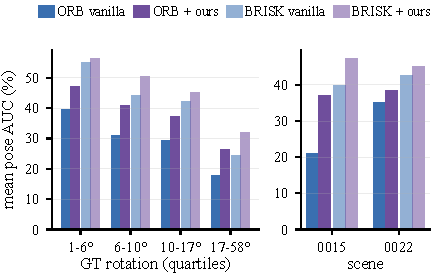
\includegraphics[width=\linewidth]{difficulty.pdf}
  \caption{\textbf{Gains across difficulty.} Mean pose AUC on MegaDepth by quartile of the ground-truth
  rotation between the two views (left) and by scene (right); \ours: mean of five seeds.}
  \label{fig:difficulty}
\end{figure}

\q{Qualitative results.} \Cref{fig:gallery} shows ORB pairs at the 95th, 80th and 60th percentile of the
per-pair gain, selected by rank rather than by eye. In the first, OpenCV's keypoints produce 17 RANSAC inliers,
none of them correct, and a pose that is off by 149$^\circ$; with \ours, 47 of 49 inliers are correct and the
error drops to 2.4$^\circ$. In the third, the response-ranked keypoints cluster on the quadriga and RANSAC
locks onto a wrong solution (141$^\circ$), while the learned selection adds keypoints on the gate and the
building behind it and recovers the pose to 16.5$^\circ$.

\begin{figure*}[t]
  \centering
  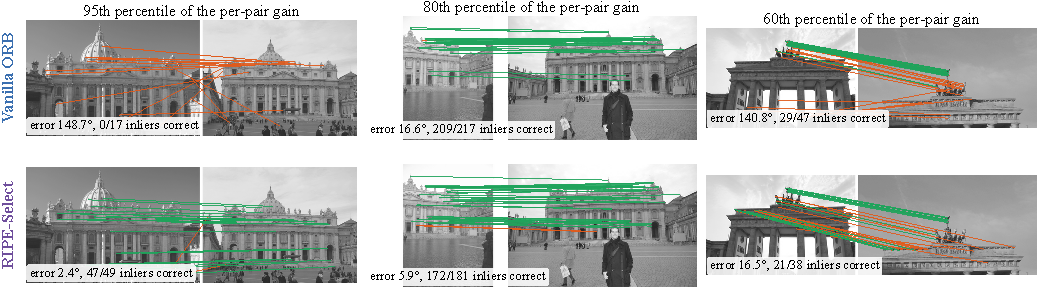
\includegraphics[width=\linewidth]{gallery.pdf}
  \caption{\textbf{Qualitative results} for ORB on MegaDepth, $K{=}2048$. Columns: pairs at the 95th, 80th and
  60th percentile of the per-pair gain of \ours (seed 0), chosen by rank. Top: OpenCV's response ranking; bottom:
  \ours. Lines: a random subset of 50 RANSAC inliers, \textcolor{good}{green} if correct (symmetric epipolar
  error below 2\,px), \textcolor{bad}{orange} otherwise. Labels: pose error and correct/total inliers.}
  \label{fig:gallery}
\end{figure*}

\begin{figure}[t]
  \centering
  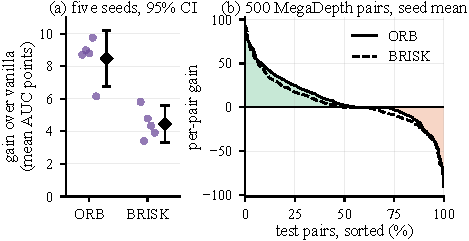
\includegraphics[width=\linewidth]{gains.pdf}
  \caption{\textbf{The gain is consistent.} (a) Gain in mean pose AUC over vanilla for each of five training
  seeds; black: mean and 95\,\% CI. (b) Per-pair gain (contribution to mean AUC, averaged over seeds), sorted;
  \textcolor{good}{green}/\textcolor{bad}{orange}: ORB pairs that improve / worsen.}
  \label{fig:gains}
\end{figure}

\begin{figure}[t]
  \centering
  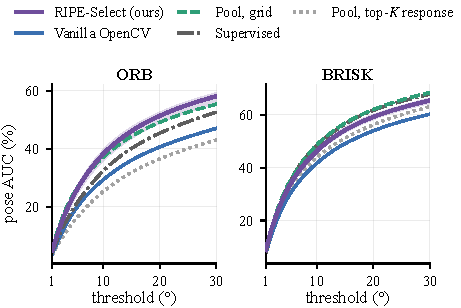
\includegraphics[width=\linewidth]{auc_curves.pdf}
  \caption{\textbf{Pose AUC vs.\ error threshold} on MegaDepth. Band: range over five \ours seeds.}
  \label{fig:auc}
\end{figure}

\q{Against published binary features.} \Cref{tab:context} sets these numbers next to published results for
binary features. Our vanilla ORB reproduces the ORB row reported by XFeat~\cite{potje2024xfeat} to within 1.7
AUC at every threshold, so the protocols agree closely. With learned selection, ORB---a 2011 detector with a
256-bit descriptor---surpasses ZippyPoint~\cite{kanakis2023zippypoint}, a learned binary feature, at every
threshold, and BRISK with \ours is ahead of both by a wide margin.

\begin{table}[t]
\centering
\footnotesize
\setlength\tabcolsep{4.2pt}
\begin{tabular}{@{}l c c c c@{}}
\toprule
MegaDepth-1500 (binary features) & @5$^\circ$ & @10$^\circ$ & @20$^\circ$ & Mean \\
\midrule
\multicolumn{5}{@{}l}{\textit{Reported by XFeat~\cite{potje2024xfeat}}} \\
ORB~\cite{rublee2011orb}                & 17.9 & 27.6 & 39.0 & 28.2 \\
ZippyPoint~\cite{kanakis2023zippypoint} & 23.6 & 34.9 & 46.3 & 34.9 \\
\midrule
\multicolumn{5}{@{}l}{\textit{Ours (top-2048, MNN, PoseLib)}} \\
ORB (OpenCV)                            & 18.8 & 29.3 & 40.6 & 29.6 \\
\quad + \ours                           & \U{24.6} & \U{38.1} & \U{51.4} & \U{38.0} \\
BRISK (OpenCV)                          & 29.0 & 41.6 & 54.0 & 41.5 \\
\quad + \ours                           & \B{32.4} & \B{46.3} & \B{59.3} & \B{46.0} \\
\bottomrule
\end{tabular}
\caption{\textbf{Binary features on MegaDepth-1500,} pose AUC (\%). XFeat's rows use all 1500 pairs, 4096
keypoints and LO-RANSAC on the essential matrix; ours use 500 evenly spaced pairs. \textbf{Bold}: best,
\underline{underlined}: second best.}
\label{tab:context}
\end{table}

\q{HPatches.} On planar HPatches (\cref{tab:main}, bottom) \ours is on par with vanilla ($\pm0.0$ mean AUC
for ORB, $+0.3$ for BRISK) and below the grid. These scenes are planar and well textured, so almost every textured
keypoint is valid and the choice among them matters little; spreading them, which the grid does by
construction, is what helps there. The policy was also trained at 1200\,px on outdoor photographs, while
HPatches images are about 480\,px.

% ============================================================================ analysis
\section{What does the policy learn?}
\label{sec:analysis}

\begin{figure*}[t]
  \centering
  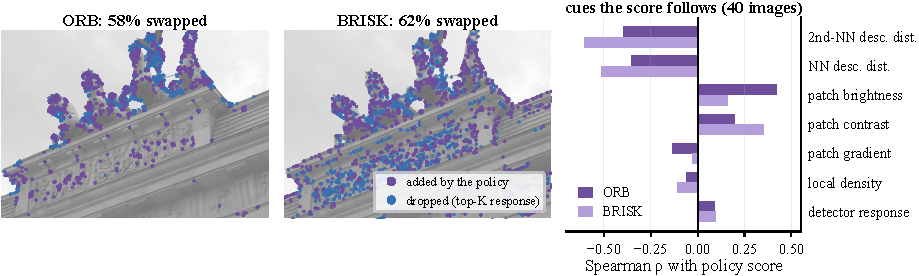
\includegraphics[width=\linewidth]{learned.pdf}
  \caption{\textbf{The policy rewrites the selection.} Left: keypoints that \ours keeps but top-$K$ response of
  the same pool does not (\textcolor{ours}{purple}), and the ones it drops (\textcolor{vanilla}{blue}), on the
  first image of \cref{fig:teaser} (zoomed). Response crowds the sculpture; the policy moves keypoints down onto
  the cornice and the facade. Right: Spearman correlation between the policy score and individual cues
  within an image, averaged over 40 MegaDepth test images. The score follows patch appearance and descriptor
  similarity; it is almost independent of the detector response that OpenCV ranks by.}
  \label{fig:learned}
\end{figure*}

\q{Is there anything to learn?} Yes. \Cref{fig:matchability} bins pool candidates by response quartile: on
MegaDepth the share that becomes a correct match only falls from 8\,\% to 4--6\,\% between the strongest and
the weakest quartile, and top-$K$ by response keeps only 40--44\,\% of the pool's correct matches.

\begin{figure}[t]
  \centering
  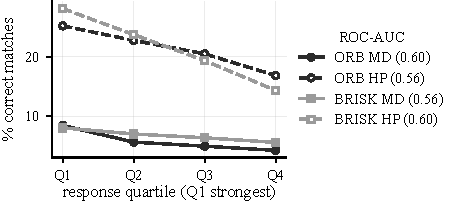
\includegraphics[width=0.92\linewidth]{matchability.pdf}
  \caption{\textbf{Response is a weak cue.} Share of candidates that become correct matches, by response
  quartile (MD: MegaDepth, HP: HPatches); legend: ROC-AUC of response as a predictor.}
  \label{fig:matchability}
\end{figure}

\q{The policy rewrites the selection.} Compared with top-$K$ response on the same pool, \ours replaces 68\,\% of
the kept keypoints for ORB and 64\,\% for BRISK (40 test images, \cref{fig:learned}). Its score is almost
uncorrelated with response ($\rho{=}0.09$). It rises with patch brightness and contrast (ORB $\rho{=}0.42$,
BRISK $\rho{=}0.35$) and, perhaps surprisingly, \emph{falls} with intra-image descriptor distinctiveness
($\rho$ between $-0.36$ and $-0.60$ for the distance to the nearest and second-nearest descriptor). A binary
descriptor far from every other one in its image may be dominated by noise, which does not repeat in the
second view; a plausible reading is that the policy prefers descriptors of structured, recurring texture. It
also slightly avoids dense clusters ($\rho{=}-0.06$ and $-0.11$ with local density). \Cref{fig:scoremap} shows
the effect on one image: response peaks on the sculpture, while the learned score is spread over the cornice
and facade.

\begin{figure}[t]
  \centering
  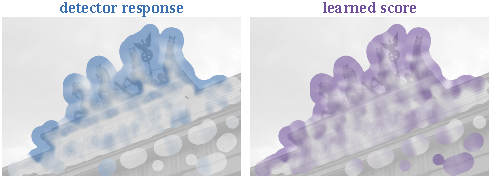
\includegraphics[width=\linewidth]{scoremap.pdf}
  \caption{\textbf{Response map vs.\ learned score map} over the ORB candidate pool of the first image of
  \cref{fig:teaser}: within-image rank of each candidate, smoothed (darker = ranked higher).}
  \label{fig:scoremap}
\end{figure}

\q{How fast does it learn?} \Cref{fig:training} tracks the validation score on the held-out \emph{Reichstag}
scene. For BRISK, all five seeds pass the response ranking (46.5) within the first 100 steps and settle at
58--60. For ORB, even the untrained policy (26--32), which keeps a nearly arbitrary subset of the larger pool,
is already well above response ranking (17.2), another sign of how much response clusters ORB's keypoints;
training then lifts the best checkpoints to 34--36. Runs take 40--90 minutes on a laptop CPU.

\begin{figure}[t]
  \centering
  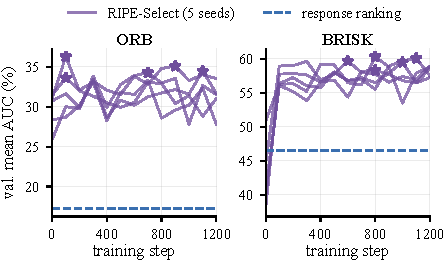
\includegraphics[width=\linewidth]{training.pdf}
  \caption{\textbf{Training curves.} Validation mean AUC on the held-out \emph{Reichstag} scene every 100
  steps, five seeds; stars: selected checkpoints. Dashed: top-$K$ response ranking on the same scene.}
  \label{fig:training}
\end{figure}

\q{More correct matches, or better-placed ones?} \Cref{tab:quality} separates the two. For BRISK, \ours raises
both: match precision (MMA@3\,px 24.7\,\% $\to$ 26.9\,\%), inlier ratio (22.2\,\% $\to$ 24.5\,\%) and the
number of positive-pair inliers (100 $\to$ 125). For ORB, precision and inlier ratio are unchanged and the
policy keeps \emph{fewer} RANSAC inliers than vanilla (137 \vs 156); the keypoints it adds are, one by one,
no more likely to match than those it drops (6.7\,\% \vs 8.1\,\% end in a correct match). Yet ORB gains
the most pose accuracy. The difference is placement: the inliers of \ours cover 9.7\,\% of the
$16{\times}16$ image cells, against 7.6\,\% for vanilla and 7.0\,\% for top-$K$ response of the same pool
(\cref{fig:coverage}). Spread-out correspondences constrain the relative pose far better than the same number
clustered on one textured object.

\finding{Trained with a per-keypoint reward and without image coordinates, the policy learns to spread its
matches over the image. For ORB this, not higher per-keypoint precision, is where the pose gain comes from.}

\begin{table}[t]
\centering
\footnotesize
\setlength\tabcolsep{2.9pt}
\begin{tabular}{@{}ll c c c c
                c c@{}}
\toprule
& & \multicolumn{3}{c}{MMA (\%)} & {Inl.} & {Cov.} & {Time} \\
\cmidrule(lr){3-5}
& & {@1\,px} & {@3\,px} & {@5\,px} & {(\%)} & {(\%)} & {(ms)} \\
\midrule
\tabinput{tables/matched_rows.tex}
\bottomrule
\end{tabular}
\caption{\textbf{Quality, coverage and cost} on MegaDepth (seed 0). MMA: share of MNN matches with
epipolar error below the threshold. Inl.: RANSAC inlier ratio. Cov.: share of $16{\times}16$ cells containing
a RANSAC inlier (50 pairs). Time: median single-thread detection and selection per image, measured in
isolation.}
\label{tab:quality}
\end{table}

\begin{figure}[t]
  \centering
  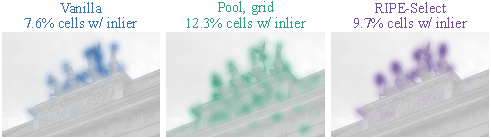
\includegraphics[width=\linewidth]{coverage.pdf}
  \caption{\textbf{Where the kept keypoints are.} Density of the 2048 kept ORB keypoints on the first image of
  \cref{fig:teaser}. Titles: share of $16{\times}16$ cells containing a RANSAC inlier, averaged over 50
  MegaDepth pairs.}
  \label{fig:coverage}
\end{figure}

\q{The grid takes the same route further.} Bucketing the pool into a grid spreads inliers even more (12.3\,\%
of cells for ORB, 17.0\,\% for BRISK) at the price of precision (ORB inlier ratio 24.0\,\% $\to$ 17.6\,\%), and
it reaches a similar pose accuracy: \ours is ahead by 0.9 for ORB and behind by 2.2 for BRISK, neither
difference significant (\cref{fig:forest}). Forcing the learned scores into the same grid does not combine the
two: it lowers ORB to 34.0, because the grid then overrides the placement the policy chose. Learning precision
and coverage \emph{jointly}---a coverage-aware reward, or a selection rule that trades the two---is the clear
next step.

\begin{figure}[t]
  \centering
  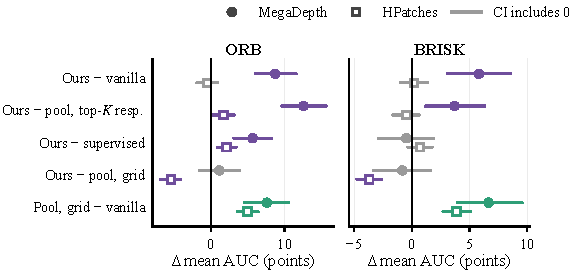
\includegraphics[width=\linewidth]{forest.pdf}
  \caption{\textbf{Paired bootstrap} differences in mean AUC with 95\,\% CIs (seed-0 policy). Grey: the
  interval includes zero.}
  \label{fig:forest}
\end{figure}

\q{Is it just the larger pool?} No. Ranking the same pool by response \emph{lowers} ORB accuracy by 3.9 AUC:
the extra low-threshold candidates pile up on the most textured regions. \ours (seed 0) beats this pool top-$K$
by +12.6 for ORB and +3.7 for BRISK, both significant (\cref{fig:forest}).

\q{Does reinforcement learning matter?} For ORB, \ours beats the supervised model trained on the same RANSAC
pseudo-labels by +5.7 [+3.1, +8.2]; for BRISK the two are equal ($-0.5$ [$-2.9$, +1.9]). The negative-pair
penalty is not the explanation: on 50 MegaDepth pairs each also matched against an image of the other scene,
\ours lowers the mean number of ORB inliers on these negative pairs only from 21.8 to 19.5, and the ratio of
positive to negative inliers is unchanged (7.0 \vs 7.1). A more likely cause is the training signal itself: RL
is rewarded for matches among \emph{sampled} subsets of the pool, exactly as at test time, so it can learn which
keypoints work \emph{together}---including where they lie---whereas the supervised labels judge each candidate in
isolation on the full pool.

\q{What does it cost?} The policy needs the larger pool and the cues. In an isolated single-thread benchmark
(median of 20 MegaDepth images) the pipeline takes 838\,ms per image for ORB and 1077\,ms for BRISK, against 20
and 81\,ms for OpenCV (\cref{fig:pareto}). About 740\,ms of this is cue computation in unoptimised Python; the MLP
takes 27--41\,ms and the final selection about 1\,ms. Most cues are box filters and nearest-neighbour counts that
map directly to C++ or a GPU.

\begin{figure}[t]
  \centering
  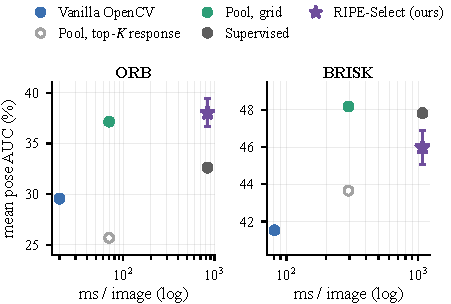
\includegraphics[width=\linewidth]{pareto.pdf}
  \caption{\textbf{Accuracy vs.\ cost} on MegaDepth. \ours: five-seed mean $\pm$ std; supervised shares its
  runtime.}
  \label{fig:pareto}
\end{figure}

% ============================================================================ limitations / conclusion
\section{Limitations}
\label{sec:limitations}
Training uses two scenes (700 images), no hyper-parameter search and one validation scene; RIPE uses the DISK
MegaDepth subset and about three GPU-days, so more training data is a natural extension. MegaDepth results use
500 of the 1500 pairs, and the ablations and bootstrap tests use seed 0. Cue computation in Python makes selection
slow. We focus on ORB and BRISK, the binary detectors behind most lightweight pipelines; applying \ours to
float-descriptor detectors such as SIFT and SURF is ongoing work.

\section{Conclusion}
\label{sec:conclusion}
Which keypoints a classical detector keeps is worth learning, and it can be learned from image-pair labels
alone. Without touching detector, descriptor or matcher, \ours lifts ORB by 8.5 and BRISK by 4.5 pose AUC on
MegaDepth-1500, consistently across seeds, and moves ORB past a learned binary feature. The policy discards the
detector's response ranking, rewrites two-thirds of the selection and, without seeing coordinates, learns to spread
its matches---the same property a hand-made grid enforces. Teaching the policy to trade precision against coverage
explicitly, and making the cues fast, are the steps that would turn this into a free upgrade for every ORB-based
system.

{
  \small
  \bibliographystyle{ieeenat_fullname}
  \bibliography{refs}
}

% ============================================================================ supplementary
\clearpage
\setcounter{page}{1}
\onecolumn
\appendix
\begin{center}
  {\Large\bfseries Supplementary Material}\\[0.4em]
  {\large Which Keypoints Should ORB Keep?}
\end{center}
\vspace{1em}

\section{Per-seed results}
\label{app:seeds}
\begin{table}[h]
\centering
\small
\begin{tabular}{@{}ll c c c c
                c c c@{}}
\toprule
& & \multicolumn{3}{c}{MegaDepth AUC} & \multicolumn{3}{c}{HPatches AUC} & {Val.} \\
\cmidrule(lr){3-5}\cmidrule(lr){6-8}
& & {@5$^\circ$} & {@10$^\circ$} & {@20$^\circ$} & {@1\,px} & {@3\,px} & {@5\,px} & {AUC} \\
\midrule
\tabinput{tables/seeds_rows.tex}
\bottomrule
\end{tabular}
\caption{\ours per training seed. Val.: best mean AUC on the held-out \emph{Reichstag} scene, used for
checkpoint selection (plain response: ORB 17.2, BRISK 46.5).}
\label{tab:seeds}
\end{table}

\section{Additional qualitative results}
\label{app:qual}
\Cref{fig:supp_brisk} shows the BRISK pair whose per-pair gain is closest to the BRISK mean gain;
\cref{fig:supp_fail} shows an ORB pair on which \ours is worse than vanilla, chosen as the pair whose loss is
closest to the mean ORB gain with opposite sign. In the failure case all three selections recover the pose
roughly (8.5--10.6$^\circ$), and \ours has more correct inliers but concentrated in a smaller region.

\begin{figure}[h]
  \centering
  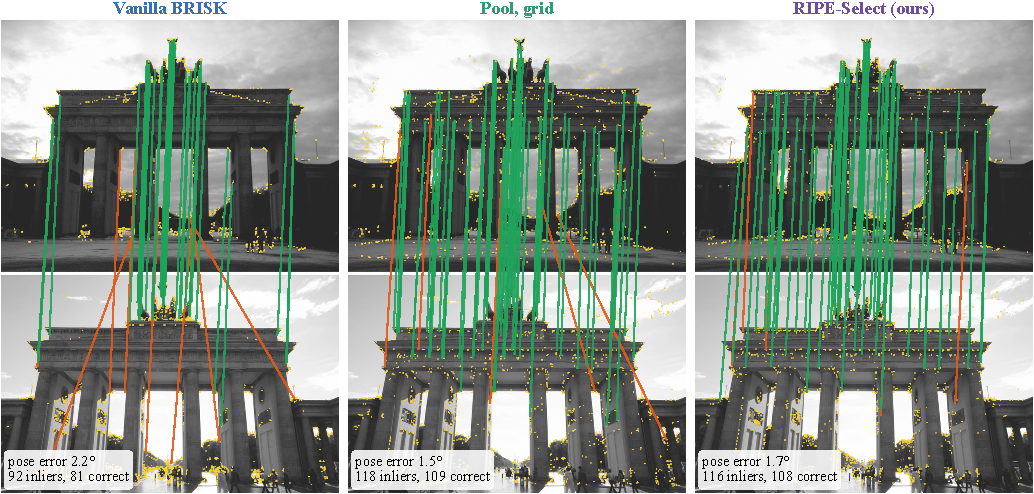
\includegraphics[width=0.85\linewidth]{supp_brisk_rep.pdf}
  \caption{BRISK, representative pair (per-pair gain 5.8 \vs mean 5.8 AUC points).}
  \label{fig:supp_brisk}
\end{figure}

\begin{figure}[h]
  \centering
  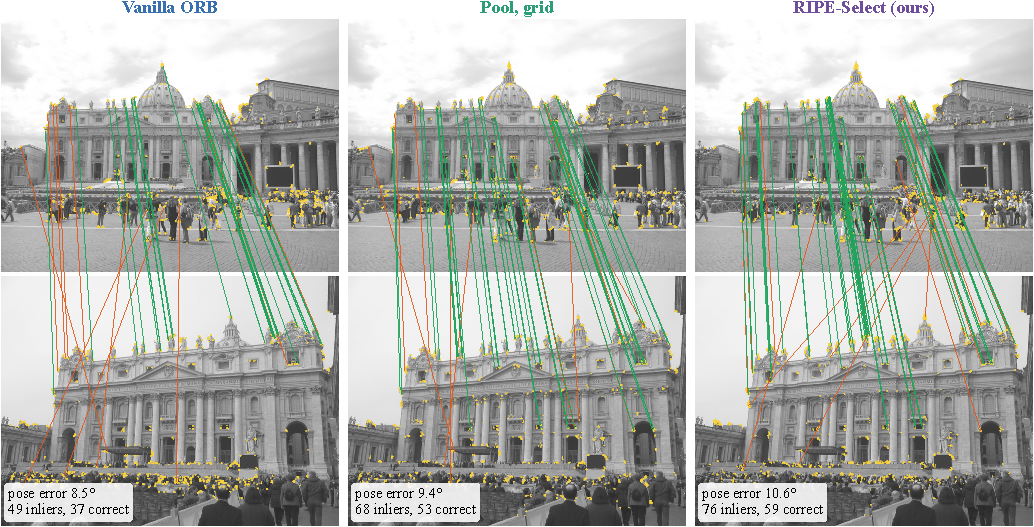
\includegraphics[width=0.85\linewidth]{supp_orb_fail.pdf}
  \caption{ORB, failure case (per-pair change $-8.6$ AUC points).}
  \label{fig:supp_fail}
\end{figure}

\section{Per-candidate cues}
\label{app:cues}
The 20 scalar cues computed for every pool candidate:
(1)~log response; (2)~log response standardised over the image; (3)~response rank in the pool; (4)~log size;
(5)~pyramid octave; (6)~layer within the octave (0 for ORB and BRISK); (7)~number of other detections within
0.5\,px; (8)~number of candidates within 16\,px; (9)~response rank among those neighbours; (10,~11)~distance to
the nearest and second-nearest other descriptor in the same image, normalised by the image median; (12)~their
ratio; (13--15)~mean intensity, intensity standard deviation and mean gradient magnitude in a box of radius
$0.75\times$ size; (16,~17)~mean and standard deviation relative to the whole image; (18)~log pool size;
(19,~20)~image mean intensity and standard deviation. They are followed by the descriptor as $\pm1$ bits (256 for
ORB, 512 for BRISK).

\section{Hyper-parameters and protocol}
\label{app:hparams}
\begin{center}
\small
\begin{tabular}{@{}ll@{}}
\toprule
Pool & $4K$ candidates (8192 at $K{=}2048$); ORB: FAST thr.\ 7, up to 8K; BRISK: AGAST thr.\ 10 (default 30) \\
Policy & MLP, inputs $\to$ 128 $\to$ 64 $\to$ 1, ReLU \\
Training & 1200 steps $\times$ 12 pairs, 50\,\% negative, $K{=}2048$, Adam with learning rate $10^{-3}$ \\
Reward RANSAC & fundamental matrix, 1.5\,px at 1200\,px, 2000 iterations \\
REINFORCE baseline & per-image mean reward \\
Validation & every 100 steps, 96 pairs of \emph{Reichstag} \\
Test RANSAC & PoseLib, 100k iterations, seed 0 \\
RANSAC threshold & tuned on vanilla: MegaDepth 1.0\,px (from 1.0, 1.5); HPatches ORB 2\,px, BRISK 4\,px (from 1, 2, 3, 4, 6) \\
Runtime & single thread, warm-up pass, median over 20 images (\texttt{timing\_benchmark.py}) \\
Policy analysis & seed-0 policies; 40 MegaDepth test images for cue correlations, 50 pairs for match rates and coverage \\
\bottomrule
\end{tabular}
\captionof{table}{Training and evaluation settings.}
\label{tab:hparams}
\end{center}

\end{document}
